% Entity-Relationship Diagram
% Diagram prompt/description: thesis 3/data/diagram_descriptions.md — fig_erd.tex
% Input this file inside a figure environment
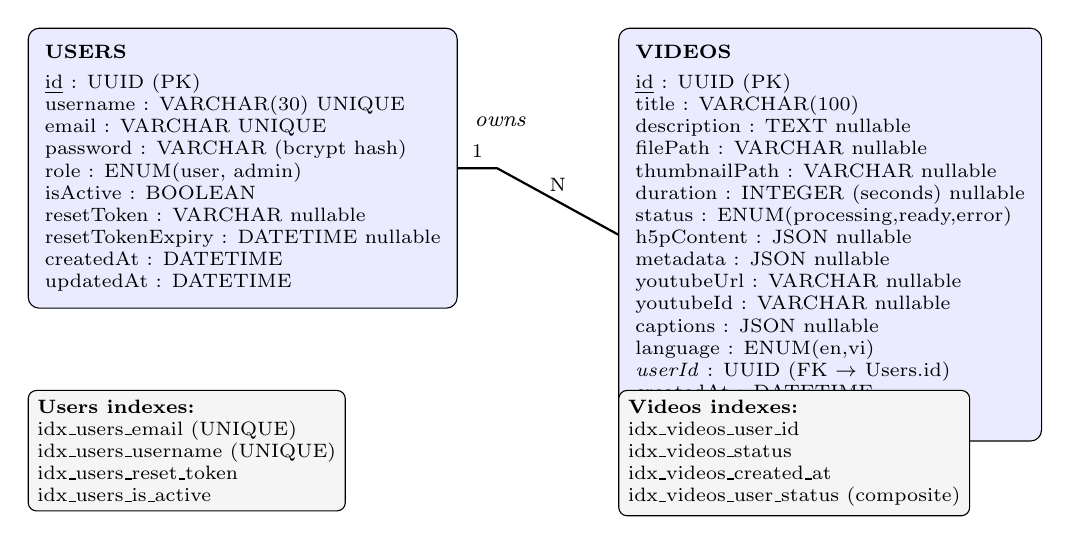
\begin{tikzpicture}[
  font=\small,
  entity/.style={draw, rounded corners=4pt, fill=blue!8,
                 minimum width=4.5cm, align=left,
                 inner sep=6pt, font=\scriptsize},
  pk/.style={font=\scriptsize\bfseries},
  fk/.style={font=\scriptsize\itshape},
]

% ── USERS entity ──────────────────────────────────────────────────────────────
\node[entity, anchor=north west] (users) at (0,0) {
  \textbf{USERS} \\[3pt]
  \underline{id} : UUID (PK) \\
  username : VARCHAR(30) UNIQUE \\
  email : VARCHAR UNIQUE \\
  password : VARCHAR (bcrypt hash) \\
  role : ENUM(user, admin) \\
  isActive : BOOLEAN \\
  resetToken : VARCHAR nullable \\
  resetTokenExpiry : DATETIME nullable \\
  createdAt : DATETIME \\
  updatedAt : DATETIME
};

% ── VIDEOS entity ─────────────────────────────────────────────────────────────
\node[entity, anchor=north west] (videos) at (7.5, 0) {
  \textbf{VIDEOS} \\[3pt]
  \underline{id} : UUID (PK) \\
  title : VARCHAR(100) \\
  description : TEXT nullable \\
  filePath : VARCHAR nullable \\
  thumbnailPath : VARCHAR nullable \\
  duration : INTEGER (seconds) nullable \\
  status : ENUM(processing,ready,error) \\
  h5pContent : JSON nullable \\
  metadata : JSON nullable \\
  youtubeUrl : VARCHAR nullable \\
  youtubeId : VARCHAR nullable \\
  captions : JSON nullable \\
  language : ENUM(en,vi) \\
  \textit{userId} : UUID (FK $\to$ Users.id) \\
  createdAt : DATETIME \\
  updatedAt : DATETIME
};

% ── Relationship line ─────────────────────────────────────────────────────────
\draw[thick] (users.east) -- node[above, font=\scriptsize]{1} ++(0.5,0)
             -- node[above, font=\scriptsize]{N} (videos.west);

% ── Relationship label ────────────────────────────────────────────────────────
\node[font=\footnotesize\itshape, fill=white] at (6.0,-1.2)
  {owns};

% ── Indexes annotation ────────────────────────────────────────────────────────
\node[draw, rounded corners=3pt, fill=gray!8,
      align=left, font=\scriptsize, anchor=north west] at (0,-4.6) {
  \textbf{Users indexes:}\\
  idx\_users\_email (UNIQUE)\\
  idx\_users\_username (UNIQUE)\\
  idx\_users\_reset\_token\\
  idx\_users\_is\_active
};

\node[draw, rounded corners=3pt, fill=gray!8,
      align=left, font=\scriptsize, anchor=north west] at (7.5,-4.6) {
  \textbf{Videos indexes:}\\
  idx\_videos\_user\_id\\
  idx\_videos\_status\\
  idx\_videos\_created\_at\\
  idx\_videos\_user\_status (composite)
};

\end{tikzpicture}
